\documentclass[]{article}
\usepackage[utf8]{inputenc}
\usepackage[T1]{fontenc}
\usepackage{xcolor}
\usepackage{listings}
\usepackage{indentfirst}
\usepackage{hyperref}
\usepackage{graphicx}
\graphicspath{ {./wykresy/} }
\usepackage{geometry}
\usepackage{multirow}
\usepackage{color, colortbl}
\usepackage[font=small,labelfont=bf]{caption}

\geometry{
	a4paper,
	total={170mm,257mm},
	left=20mm,
	top=20mm,
}
\hypersetup{
	colorlinks=true,
	linkcolor=blue,
	filecolor=magenta,      
	urlcolor=cyan,
}

%%
%% Julia definition
%%
\lstdefinelanguage{Julia}%
{morekeywords={abstract,break,case,catch,const,continue,do,else,elseif,%
		end,export,false,for,function,immutable,import,importall,if,in,%
		macro,module,otherwise,quote,return,switch,true,try,type,typealias,%
		using,while},%
	sensitive=true,%
	alsoother={\$},
	morecomment=[l]\#,%
	morecomment=[n]{\#=}{=\#},%
	morestring=[s]{"}{"},%
	morestring=[m]{'}{'},%
}[keywords,comments,strings]%
\lstset{%
	language         = Julia,
	basicstyle       = \ttfamily,
	keywordstyle     = \bfseries\color{blue},
	stringstyle      = \color{magenta},
	commentstyle     = \color{gray},
	showstringspaces = false,
}


%opening
\title{Obliczenia naukowe. Lista nr 4. Sprawozdanie.}
\author{Kacper Szatan, nr 236478}
\date{December 8, 2019}
\begin{document}
\maketitle
\section{Zadanie 1}
\subsection{Opis problemu}
W zadaniu pierwszym należało zaimplementować funkcję obliczającą ilorazy różnicowe. Jako dane wejściowe otrzymujemy tablicę węzłów wraz z ich odpowiadającymi wartościami (również w formie tablicy) w funkcji $f$, którą chcielibyśmy interpolować. Na wyjściu mamy zwracać tablicę ilorazów różnicowych potrzebną do interpolacji. Całość należało zrealizować bez używania tablicy dwuwymiarowej.
\subsection{Realizacja}
Iloraz różnicowy zapisujemy jako wzór rekurencyny w następujący sposób:
\begin{equation}
f[x_i] = f(x_i)
\end{equation}
\begin{equation}
f[x_i, x_{i+1}, \ldots, x_{i+j-1}, x_{i+j}] = \frac{f[x_{i+1}, x_{i+2}, \ldots, x_{i+j - 1}, x_{i+j}] - f[x_{i}, x_{i+1}, \ldots, x_{i+j-2}, x_{i+j-1}]}{x_{i+j} - x_i}
\end{equation}
Warty odnotowania jest fakt, że ilorazy różnicowe nie zależą od kolejności węzłów. Istotną informacją jest również, że iloraz różnicowy $f[x_0, x_1, \ldots x_{n-1}, x_n]$ jest współczynnikiem interpolowanej funkcji $f$, stojącym przy składniku $x^n$.

Chcąc wyznaczyć wszystkie ilorazy różnicowe, to jest $f[x_0], f[x_0, x_1], \ldots, f[x_0, \ldots, x_n]$ budujemy tablice kolumna po kolumnie (od lewej do prawej). Korzystamy przy tym ze wzoru rekurencyjnego. Dla skrócenia zapisu przyjmijmy notacje $v_{i,j} = f[x_i, x_{i+1}, \ldots, x_{i+j-1}, x_{i+j}],\:\: i + j \le n$. Tablica jest postaci:
\begin{table}[h]
	\centering
	\begin{tabular}{c c c c c} 
		\hline
		 \rowcolor{blue!20}$v_{0,0}$ & $v_{0,1}$ & \ldots & $v_{0,n - 1}$ & $v_{0,n}$\\
		 $v_{1,0}$ & $v_{1,1}$ & \ldots & $v_{1,n - 1}$ &\\
		 \vdots & \vdots & \vdots  &   & \\
		 $v_{n - 2,0}$ & $v_{n - 2,1}$ & $v_{n - 2,2}$ & &\\
		 $v_{n - 1,0}$ & $v_{n - 1,1}$ & & &\\
		 $v_{n,0}$ & & & &\\
		
		\hline
	\end{tabular}
\end{table} 
\\
W tym podejściu używamy tablicy dwuwymiarowej, którą sukcesywnie zapełniamy. Jednakże interesujące nas wartości ilorazów znajdują się tylko w pierwszym rzędzie tej tablicy. A wykorzystujemy jedynie połowę miejsca zalokowanego na tablice dwuwymiarową. Zauważmy, że wyliczając wartości kolumny opieramy się tylko o wyliczenia z poprzedniej kolumny, a cała reszta tablicy nie jest używana. Drugim spostrzeżeniem jest to, że każda kolejna kolumna ma o jeden mniej składnik niż następna. Korzystając z tego możemy zaproponować sposób wyliczania ilorazów róznicowych za pomocą tablicy jednowymiarowej o długości n. 
Na poczatku zmodyfikujmy miejsca zapisu w naszej tablicy dwu wymiarowej tak aby interesujące nas ilorazy różnicowe pojawiły się nie w pierwszym rzędzie macierzy a na jej przękątnej. Można to porównać do "opuszczenia wiszących" kolumn na "dno" tablicy \textit{(zob. Table 1)}. 


\begin{table}[h]
	\centering
	\begin{tabular}{c c c c c} 
		\hline
		\cellcolor{blue!20}$v_{0,0}$ & & & &\\
		$v_{1,0}$ & \cellcolor{blue!20}$v_{0,1}$ & & &\\
		$v_{2,0}$ & $v_{1,1}$ & \cellcolor{blue!20}$v_{0,2}$& &\\
		\vdots & \vdots & \vdots  &  & \\
		%$v_{n - 2,0}$ & $v_{n - 3,1}$ & \ldots & &\\
		$v_{n - 1,0}$ & $v_{n - 2,1}$ & \ldots & \cellcolor{blue!20}$v_{0,n - 1}$&\\
		$v_{n,0}$ & $v_{n - 1,1}$ & \ldots & $v_{1,n - 1}$ & \cellcolor{blue!20}$v_{0,n}$\\
		
		\hline
	\end{tabular}
	\caption{Wizualizacaj zmodyfikowanej macierzy z innym podejściem miejsca zapisu.}
\end{table}

Wykorzystując nasze pierwsze spostrzeżenie możemy ograniczyć się jedynie do jednowymiarowej tablicy przez "spłaszczenie" macierzy do jednej pierwszej kolumny. W każdym kroku wyniki z wyliczanej kolumy będą nadpisywały poprzednią (i jedyną kolumnę). Wtedy po zakończeniu obliczeń dostaniemy wektor długości n+1, który będzie zawierał interesujące nas ilorazy różnicowe. Aby osiągnąć interesujący nas zapis, w pierwszym kroku wypełniamy nasz wektor wartościami zadanych  węzłów. Następnie w pętli wyliczamy wartości następnych kolumn zaczynając "od dołu" i zapisując wartość w "najniższej" komórce, która brała udział w wyliczeniach. Taki sposób zapewni nam nadpisywanie danych, które już nie będą potrzebne do obliczeń. Poniżej zamieszczono pseudokod realizujące omówiony algorytm.
\\
\hrule
\begin{lstlisting}
function iR(x, f)
 fx <== kopia(f) #Pierwszy krok
 # f[x0] jest juz dobrze ustawione dlatego iteracje petli zaczynamy od 2	
 for i <== 2, dlugosc(fx) # w kazdym obrocie petli zwiekszamy i o jeden
 #petla konczy sie gdy j = dlugosc(fx)
  for j <== dlugosc(fx), i # w kazdym obrocie petli zmniejszami j o jeden
  #petla konczy sie gdy j = i, tutaj zapewniamy liczenie "od dolu"
   fx[j] = (fx[j] - fx[j - 1]) / (x[j] - x[j - i + 1])

 return fx
end
\end{lstlisting}
\hrule
\section{Zadanie 2}
\subsection{Opis problemu}
W zadaniu drugim należało zaimplementować funkcję, która oblicza wartość wielomianu interpolacyjnego stopnia $n$ w postaci Newtona $N_n(x)$ w punkcie $x=t$. Należało to zrealizować w czasie $O(n)$, za pomocą uogólnionego algorytmu Hornera.
\subsection{Realizacja}
Wielomian interpolacyjny w postaci Newtona możemy zapisać następująco:
\[ N_n(x) =  \sum_{i = 0}^{n}(f[x_0, x_1, \ldots, x_i] \prod_{j = 0}^{i - 1}(x - x_j) ) \]
Korzystając z uogólnionego algorytmu Hornera możemy ten wielomian przedstawić za pomocą wzorów.
\begin{equation}
	N_n(x) := w_0(x)
\end{equation} 
\begin{equation}
 w_n(x) := f[x_0, x_1, \ldots, x_n]
\end{equation} 
\begin{equation}
w_i(x) := f[x_0, x_1, \ldots, x_i] + (x-x_i)*w_{i+1}(x)\:\:\: (i = n-1, \ldots, 0)
\end{equation} 


Wyliczanie wartości interpolowanego wielomianu w $x = t$ za pomocą roszerzonego algorytmu  Hornera gwarantuje nam złożoność czasową $O(n)$, gdyż wykonujemy jedynie $n$ mnożeń, i $n$ dodawań, i $n$ odejmowań.

Algorytm, który realizuje cel zadania, w pierwszym kroku przypisuje zmiennej iloraz różnicowy, z ostatniej komórki wektora $fx$. Jest to współczynnik stojący przy najwyższej potędze w interpolowanym wielomianie. Czyli realizujemy tym krokiem równanie $(4)$. Następnie w pętli korzystamy z równania $(5)$, wynik przypisując naszej zmiennej i używamy jej przy następnym obrocie pętli. Gdy wykonamy $n-1$ obrotów pętli w naszej zmiennej otrzymamy wartość interpolowanego wielomianu. Poniższy pseudo kod realizuje omówiony algorytm:    
\\
\hrule
\begin{lstlisting}
function wN(x, fx, t)
 v_in_t <== fx[length(fx)] # ostatnia komorka wektora ilorazow roznicowych
 for i <== length(fx)-1, 1 # petla obraca sie az i = 1
 # i zmniejsza sie o jeden w kazdym obrocie petli
  v_in_t = fx[i] + (t - x[i]) * v_in_t #realizacja wzoru nr (5) 
 
 return v_in_t 
end
\end{lstlisting}
\hrule
\section{Zadanie 3}
\subsection{Opis problemu}
Mając podane współczynniki wielomianu interpolacyjnego w postacie Newtona $c_0 = f[x_0], c_1 = f[x_0, x_1], \ldots, c_n = f[x_0, x_1, \ldots, x_n]$, a także węzły $x_0, x_1, \ldots, x_n$ należało zaimplementować funkcję obliczającą wspołczynniki tego wielomianu w postaci naturalnej, w czasie $O(n^2)$. 
\subsection{Realizacja}
W celu znalezienia sposobu wyznaczenia wspołczynników wielomianu w postaci naturalnej skorzystano z uogólnionego algorytmu Hornera. Łatwo możemy zauważyć, że $c_n = a_n$. Zatem mamy już punkt wyjściowy algorytmu, który w pierwszym kroku przypisuje wektorowi wspołczyników naturalnych $a[]$ wartość $c_n$ w ostatniej komórce $a$. Następnie rozpoczynamy główną pętlę zaczynając od $n-1$ i schodząc w dół, w której przypisujemy $a[i] = c_i$. Po tej operacji rozpoczynamy pętlę uaktualniającą obecny stan wektora współczynników naturalnych zaczynającą od ostatnio wstawionego wezła do przed ostatniego współczynnika. Jest to realizowane z pomocą uogólnionego algorytmu Hornera. po przejściu pętli uaktualniającej otrzymujemy współczynniki naturalne dla aktualnie rozpatrywanych węzłów. Gdy rozpatrzymy waszystkie węzły otrzymamy interesujący nas wynik. Poniżej zaprezentowano pseudokod realizujący pomysł tego algorytmu.   
\\
\hrule
\begin{lstlisting}
function n(x, fx)
 for i <== length(fx) : -1 : 1   # petla schodzi w dol co jeden
  a[i] <== fx[i]           # dodanie wezla do rozpatrywania
  for j <== i , length(fx) - 1  # petla obraca sie az j = dlugosci fx - 1      
   # uaktualnianie wektora a dla nowo dodanego wezla
   a[j] <== a[j] - x[i] * a[j + 1] 

return a
end
\end{lstlisting}
\hrule
\section{Zadanie 4}
\subsection{Opis problemu}
Celem zadania jest zkonstruowanie metody, która pozwoli nam na stworzenie wykresu funkcji interpolowanej oraz jej wielomianu interpolującego. Korzystając przy tym z wcześniej zaimplementowanych funkcji co pozwala nie wyznaczać jawnie postaci tego wielomianu. Na wejściu podajemy anonimową funkcję, którą chcemy interpolować, przedział interpolacji oraz stopien wielomianu iterpolacyjnego, który chcemy otrzymać. W interpolacji należało zastosować węzły równoodległe dane wzorem: $ x_k = a + kh, \:\: h = (b - a)/n, \:\:  k = 0, 1, ..., n$, gdzie $a$ jest początkiem przedziału, $b$ jego końcem, a $n$ liczbą węzłów.
\subsection{Realizacja}
Na początku wyznaczono węzły na, których będzie się opierał wielomian interpolacyjny. Wiemy, że interpolując z wykorzystaniem $n$ węzłów, otrzymamy wielomian conajwyżej $n-1$ stopnia. Dlatego musimy oprzeć się na $n+1$ punktach. Po wyliczeniu równoodległych węzłów wraz z odpowiadającymi im wartościami zostają obliczone ilorazy różnicowe za pomocą funkcji z zadania pierwszego. Następnie dzięki funkcji z zadania 2 jesteśmy wstanie obliczać wartość wielomianu interpolacyjnego w punkcie, bez wyznaczania jego jawnej postaci, a korzystając jedynie z wcześniej wyznaczonych węzłów oraz ilorazów różnicowych. Na koniec rysowany jest wykres z orginalną funkcją oraz jej interpolacją. Aby wykresy były bardziej precyzyjne zwiększono próbkowanie przy rysowaniu wykresów. 
\section{Zadanie 5}
\subsection{Opis problemu}
W zadaniu piątym należało przetestować zaimplementowane funkcję z zadania 4 na przykładach:
\begin{itemize}
	\item $f(x) = e^x$, na przedziale $[0, 1]$ dla stopnia wielomianu $n \epsilon \{5, 10, 15\}$
	\item $g(x) = x^2 * sin(x)$, na przedziale $[-1, 1]$ dla stopnia wielomianu $n \epsilon \{5, 10, 15\}$
\end{itemize}
\subsection{Wyniki}

\begin{minipage}{0.47\linewidth}
	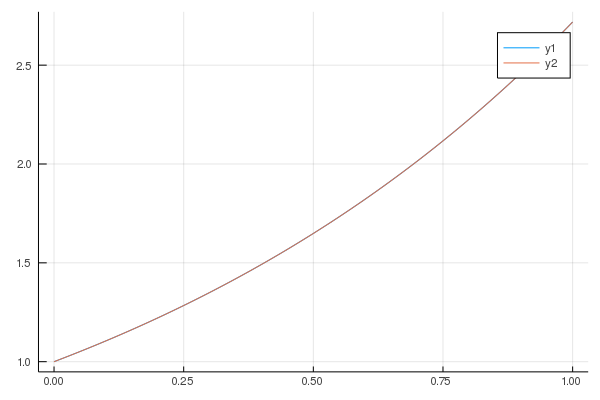
\includegraphics[width=\linewidth]{z5p1.png}
	\captionof{figure}{$f(x) = e^x$, na przedziale $[0, 1]$ dla stopnia wielomianu $n = 5$. Oryginalna funkcja linia niebieska. Wielomian interpolacyjny linia czerwona.}
\end{minipage}
\begin{minipage}{0.47\linewidth}
	
	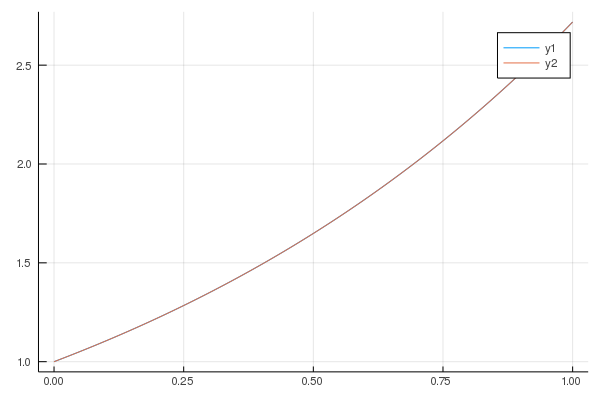
\includegraphics[width=\linewidth]{z5p2.png}
	\captionof{figure}{$f(x) = e^x$, na przedziale $[0, 1]$ dla stopnia wielomianu $n = 10$. Oryginalna funkcja linia niebieska. Wielomian interpolacyjny linia czerwona.}
\end{minipage}

\begin{minipage}{0.47\linewidth}
	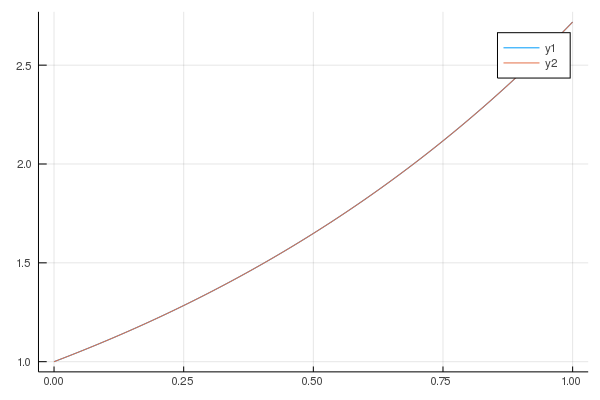
\includegraphics[width=\linewidth]{z5p3.png}
	\captionof{figure}{$f(x) = e^x$, na przedziale $[0, 1]$ dla stopnia wielomianu $n = 15$. Oryginalna funkcja linia niebieska. Wielomian interpolacyjny linia czerwona.}
\end{minipage}
\begin{minipage}{0.47\linewidth}
	
	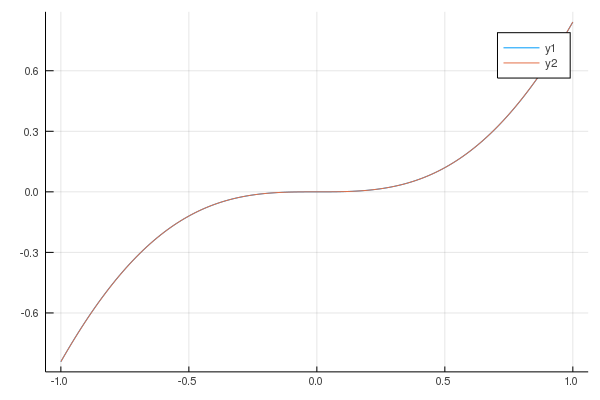
\includegraphics[width=\linewidth]{z5p4.png}
	\captionof{figure}{$g(x) = x^2 * sin(x)$, na przedziale $[-1, 1]$ dla stopnia wielomianu $n = 5$. Oryginalna funkcja linia niebieska. Wielomian interpolacyjny linia czerwona.}
\end{minipage}

\begin{minipage}{0.47\linewidth}
	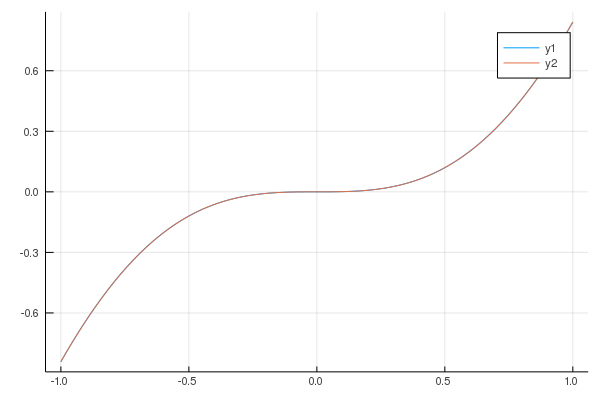
\includegraphics[width=\linewidth]{z5p5.png}
	\captionof{figure}{$g(x) = x^2 * sin(x)$, na przedziale $[-1, 1]$ dla stopnia wielomianu $n = 10$. Oryginalna funkcja linia niebieska. Wielomian interpolacyjny linia czerwona.}
\end{minipage}
\begin{minipage}{0.47\linewidth}
	
	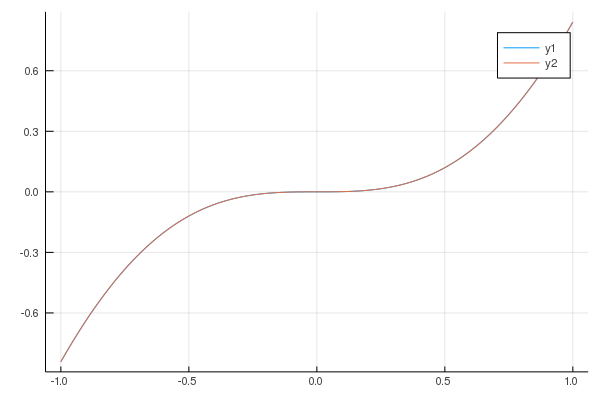
\includegraphics[width=\linewidth]{z5p6.png}
	\captionof{figure}{$g(x) = x^2 * sin(x)$, na przedziale $[-1, 1]$ dla stopnia wielomianu $n = 15$. Oryginalna funkcja linia niebieska. Wielomian interpolacyjny linia czerwona.}
\end{minipage}
\subsection{Wnioski}
W żadnym z przedstawionych przypadków nie było widać lini niebieskiej (oryginalna funkcja), która została całkowicie pokryta przez linię interpolującego wielomianu. To znaczy, że funkcja z zadania 4 bardzo dobrze interpoluje testowe przykłady. Zastosowanie węzłów równoodlgłych do interpolacji sprawdza się w tych przypadkach. Wartości wielomianu interpolującego są bardzo bliskie faktycznym wartościom funkcji w opowiadających punktach.
\section{Zadanie 6}
\subsection{Opis problemu}
W zadaniu szóstym należało przetestować zaimplementowane funkcję z zadania 4 na przykładach ilustrujących zjawisko rozbieżności:
\begin{itemize}
	\item $f(x) = |x|$, na przedziale $[-1, 1]$ dla stopnia wielomianu $n \epsilon \{5, 10, 15\}$
	\item $g(x) = \frac{1}{1+x^2}$, na przedziale $[-5, 5]$ dla stopnia wielomianu $n \epsilon \{5, 10, 15\}$
\end{itemize}
\subsection{Wyniki}
\begin{minipage}{0.47\linewidth}
	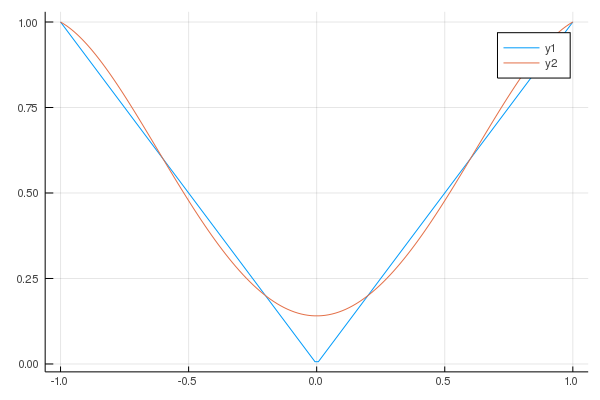
\includegraphics[width=\linewidth]{z6p1.png}
	\captionof{figure}{$f(x) = |x|$, na przedziale $[-1, 1]$ dla stopnia wielomianu $n = 5$. Oryginalna funkcja linia niebieska. Wielomian interpolacyjny linia czerwona.}
\end{minipage}
\begin{minipage}{0.47\linewidth}
	
	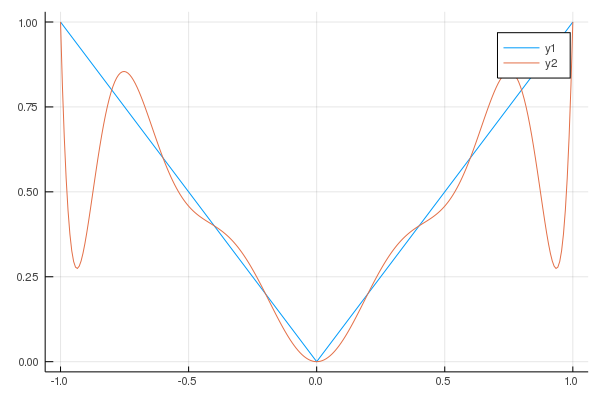
\includegraphics[width=\linewidth]{z6p2.png}
	\captionof{figure}{$f(x) = |x|$, na przedziale $[-1, 1]$ dla stopnia wielomianu $n = 10$. Oryginalna funkcja linia niebieska. Wielomian interpolacyjny linia czerwona.}
\end{minipage}

\begin{minipage}{0.47\linewidth}
	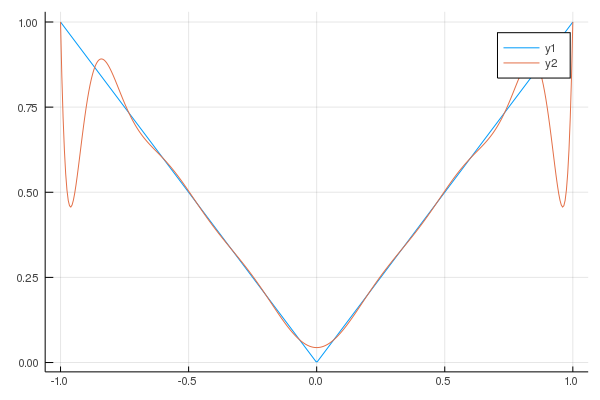
\includegraphics[width=\linewidth]{z6p3.png}
	\captionof{figure}{$f(x) = |x|$, na przedziale $[-1, 1]$ dla stopnia wielomianu $n = 15$. Oryginalna funkcja linia niebieska. Wielomian interpolacyjny linia czerwona.}
\end{minipage}
\begin{minipage}{0.47\linewidth}
	
	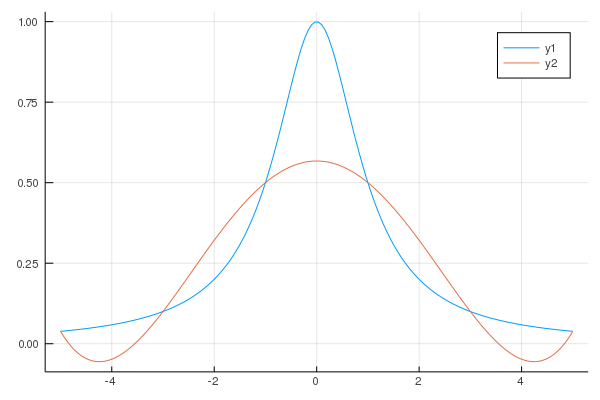
\includegraphics[width=\linewidth]{z6p4.png}
	\captionof{figure}{$g(x) = \frac{1}{1+x^2}$, na przedziale $[-5, 5]$ dla stopnia wielomianu $n = 5$. Oryginalna funkcja linia niebieska. Wielomian interpolacyjny linia czerwona.}
\end{minipage}

\begin{minipage}{0.47\linewidth}
	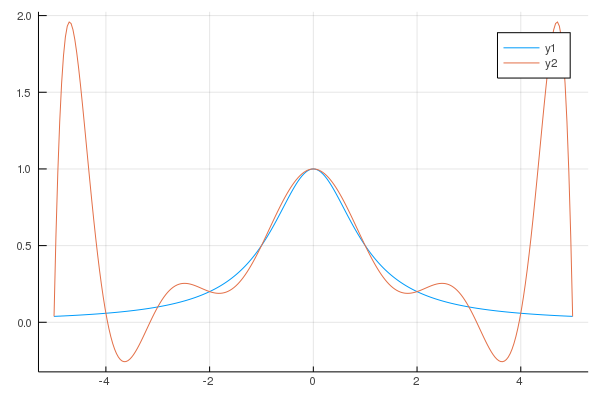
\includegraphics[width=\linewidth]{z6p5.png}
	\captionof{figure}{$g(x) = \frac{1}{1+x^2}$, na przedziale $[-5, 5]$ dla stopnia wielomianu $n = 10$. Oryginalna funkcja linia niebieska. Wielomian interpolacyjny linia czerwona.}
\end{minipage}
\begin{minipage}{0.47\linewidth}
	
	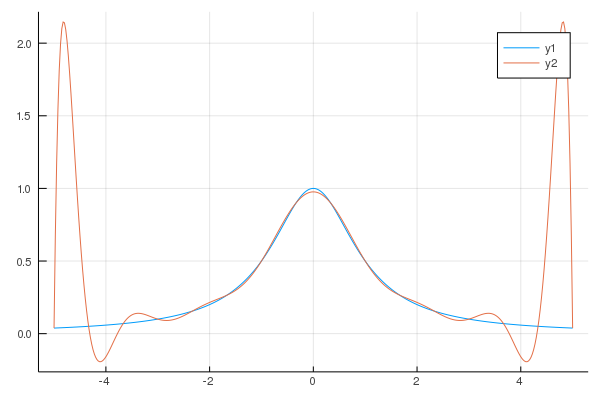
\includegraphics[width=\linewidth]{z6p6.png}
	\captionof{figure}{$g(x) = \frac{1}{1+x^2}$, na przedziale $[-5, 5]$ dla stopnia wielomianu $n = 15$. Oryginalna funkcja linia niebieska. Wielomian interpolacyjny linia czerwona.}
\end{minipage}
\subsection{Wnioski}
Analizując wykresy zauważamy dosyć interesujące zjawisko rozbieżności. Zwiększając liczbę węzłów, na których oparty jest wielomian interpolacyjny oczekujemy zwiększenia dokładności interpolacji. Zamiast tego otrzymujemy wręcz przeciwny efekt, który objawia się bardzo silnym zaburzeniem na końcach rozpatrywanych przedziałów. Jest to tak zwany efekt Rungego. Wynika on z natury wielomianów wysokiego stopnia opartych o równo odległe węzły. Duży stopień wielomianu sprawia, że wielomian chce szybko "uciec" w stronę nieskończoności. A jednocześnie posiada sporo zer, które starają się przyciągnąć go w strone prawdziwych wartości. Dlatego otrzymujemy takie zaburzenia. Rozwiązaniem tego problemu jest oparcie wielomianu o węzły Czebyszewa. Są one gęściej rozłożone na krańcach przedziału co pozwala na silniejsze "uwiązanie" wielomianu do interpolowanej funkcji w miejscach narażonych na zaburzenie. Dodatkowym problemem funkcji $f(x) = |x|$ jest to, że ma nieciągłą pochodną co również powoduje ten efekt rozbieżności. 
\end{document}